\section{Auswertung}
\label{sec:Auswertung}
In der Auswertung werden die Rechnungen, Plots und Fit-Funktionen mit \cite{matplotlib}, \cite{numpy}, \cite{scipy} und \cite{uncertainties} durchgefürht bzw. erstellt.
\subsection{Fehlerrechnung}
\label{sec:fehlerrechnung}
%\subsection{Mittelwert}
Zur Verarbeitung der Messunsicherheiten werden außerdem die folgenden Fomreln verwendet: 
Der Mittelwert wird mithilfe von

\begin{equation}
\bar{x} = \frac{1}{N} \sum_{i=1}^{N} x_i.
\label{eqn:mittelwert}
\end{equation}
bestimmt.
%\subsection{Standardabweichung}
Die Standardabweichung wird anhand von
\begin{equation}
\sigma = \sqrt{\frac{1}{N - 1} \sum_{i=1}^{N} \left( x_i - \bar{x}_N \right)^2}.
\label{eqn:standardabweichung}
\end{equation}
berechnet.
%%\subsubsection{Standardabweichung des Mittelwerts}
Die Standardabweichung des Mittwertes wird mithilfe von 
\begin{equation}
\Delta \bar{x} = \frac{\sigma}{\sqrt{N}}
\label{eqn:standardmittelwert}
\end{equation}
bestimmt.
%%\subsection{Gaußsche Fehlerfortpflanzung}
%Die Abweichung eines Wertes, der sich aus experimentell bestimmten Parametern ergibt, kann mithilfe der Gaußschen Fehlerfortpflanzung 
%\begin{equation}
%\Delta f = \sqrt{\sum_{i=1}^{N} \left( \frac{\partial f}{\partial x_i} \right)^2 \cdot (\Delta x_i)^2}
%\label{eqn:fehlerfortpflanzung}
%\end{equation}
%ermittelt werden.









\subsection{Berechnung der theoretischen Stabilitätsbedinung}
\label{subsec:theostab}
Zunächst wird die theoretische Stabilitätsbedingung von der Anordnung mit zwei konkaven Spiegeln mit gleichem Krümmungsradius $r$ berechnet.
Nach \autoref{eqn:g} gilt $g_1 g_2 = g_1^2 = 1 - 2 \frac{L}{r} + \left(\frac{L}{r}\right)^2$.
Es ergibt sich also eine quadratische Abhängigkeit von $L$.
Die maximale Länge des Resonators ist nach \autoref{eqn:stabbed} $L_{\mathrm{max}}=\qty{2.8}{\meter}$.
Diese ist für $r=\qty{1400}{\milli\meter}$ in \autoref{fig:theostab} dargestellt. 
\\
Für die Anordnung mit einem Planspiegel und einem konkaven Spiegel mit Krümmungsradius $r$ ergibt sich nach \autoref{eqn:g} $g_1 g_2 = 1 \cdot g_2 = 1 - \frac{L}{r}$, da für den Planspiegel der Krümmungsradius als $\infty$ angenommen wird und somit $g_1 = 1$ ist.
Hierbei ergibt sich also eine lineare Abhängigkeit von $L$.
Nach \autoref{eqn:stabbed} ergibt sich eine maximale Resonatorlänge von $L_{\mathrm{max}}=\qty{1.4}{\meter}$.
Auch diese Stabilitätsbedingung ist für $r=\qty{1400}{\milli\meter}$ in \autoref{fig:theostab} dargestellt. 

\begin{figure}
  \centering
  
\includegraphics[width=0.5\textwidth]{content/images/theostab.pdf}
  \caption{Theoretisch berechnete Stabilitätsbedingung für eine Anorndung mit zwei konkaven Spiegeln sowei eine Anordnung mit einem Planspiegel und einem konkaven Spiegel.}
  \label{fig:theostab}
\end{figure}











\subsection{Auswertung der Messung der Transversalmoden}
\label{subsec:tem}
Zunächst wird das Ergebnis der Messung der Transversalmode TEM00 untersucht. 
Die genauen Messwerte sind in \autoref{tab:tem00} dargestellt. 
In \autoref{fig:tem00} sind die Werte in einem Diagram dargestellt.
Außerdem ist wird Fit-Funktion der Form \autoref{eqn:tem00} auf die Werte angewandt.
Die Parameter des Fits lauten:
\begin{align*}
    w= \\
    x_0= \\
    A_{00}= \\
    C= \, . 
\end{align*}
Dabei wird für den Fit der zu $I_{\mathrm{dunkel}}=\qty{0.009}{\micro\ampere}$ gemessene Dunkelstrom jeweils von den einzelnen Werten abgezogen. 
\begin{figure}
  \centering
  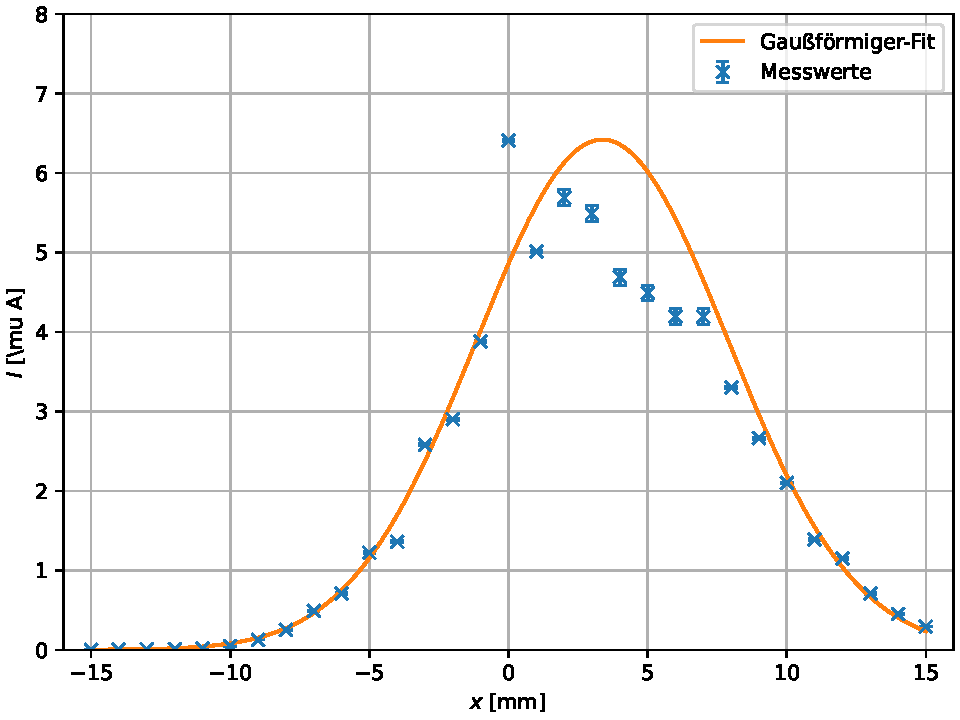
\includegraphics[width=0.5\textwidth]{content/images/tem00.pdf}
  \caption{Darstellung der Messwerte der TEM00-Mode mit gaußförmiger Fit-Funktion.}
  \label{fig:tem00}
\end{figure}
Es wird deutlich, dass die Messwerte trotz leichter Abweichungen der erwarteten Gaußverteilung entsprechen.
\\
Analog werden die Messwerte der TEM01-Mode, welche in \autoref{tab:tem01} dargestellt sind, ausgewertet. 
Sie sind in \autoref{fig:tem01} zu erkennen. 
Dabei wird eine Fit-Funktion der Form \autoref{eqn:tem01} angewand.
Die Parameter des Fits lauten:
\begin{align*}
    w= \\
    x_0= \\
    A_{00}= \\
    C=  \, .
\end{align*}
Auch hier wird zuvor der Dunkelstrom abegezogen.

\begin{figure}
  \centering
  
\includegraphics[width=0.5\textwidth]{content/images/tem01.pdf}
  \caption{Darstellung der Messwerte der TEM01-Mode mit Fit-Funktion der Form Gaußglocke mal Hermite-Polynom $H_1$.}
  \label{fig:tem01}
\end{figure}
Auch hier entsprechen die Messwerte der erwarteten Verteilung. 
Allerdings ist zu erkennen, dass die beiden Peaks unterschiedlich groß sind. 
Die Abweichungen sind bei der TEM01-Mode also deutlicher. 









\subsection{Auswertung der Messung der Stabilitätsbedingung}
\label{subsec:stab}
Zunächst wird die Messung der Stabilitätsbedinung bei einer Anordnung des Resonators mit zwei konkaven Spiegeln untersucht. 
Die Messwerte sind in \autoref{tab:konkon} eingetragen. 
Eine graphische Darstellung ist in \autoref{fig:konkon} dargestellt. 
Dabei wird eine quadratische Fit-Funktion 
\begin{equation*}
  f\left(x\right)=ax^2 + bx +c
\end{equation*}
durch die Werte gelegt.
Diese hat die Parameter
\begin{align*}
    a= \\
    b= \\
    c= \, .
\end{align*}
Auch hier muss zuvor der Dunkelstrom jeweils von den Werte abgezogen werden.
Diese wurde für das hier verwendete Gerät zu $I_{\mathrm{dunkel}}=\qty{-0.037}{\milli\watt}$ gemessen.
\begin{figure}
  \centering
  
\includegraphics[width=0.5\textwidth]{content/images/konkon.pdf}
  \caption{Darstellung der Messung der Stabilitätsbedingung bie zwei konkaven Spiegeln mit quadratischer Fit-Funktion.}
  \label{fig:konkon}
\end{figure}
Es wird deutlich dass die Proportionalität der in \autoref{subsec:theostab} bestimmten Proportionalität der Stabilitätsbedingung entspricht. 
Eine maximale Länge kann leider nicht bestimmt werden, da der Aufbau dazu nicht lang genug ist. 
\\
Die Ergebnisse bei Anordnung eines Planspiegels und eines konkaven Spiegels sind in \autoref{tab:plankon} zu finden. 
In \autoref{fig:plankon} sind diese graphisch dargestellt. 
Hier wird ein linearer Fit der Form
\begin{equation*}
  f\left(x\right) = ax + b
\end{equation*}
angewand.
Es ergeben sich die Parameter
\begin{align*}
  a= \\
  b= \, .
\end{align*}
Erneut wird hier vorher der Dunkelstrom von jedem Messwert abgezogen. 
\begin{figure}
  \centering
  
\includegraphics[width=0.5\textwidth]{content/images/plankon.pdf}
  \caption{Darstellung der Messung der Stabilitätsbedingung bei einem Planspiegel und einem konkaven Siegel mit linearer Fit-Funktion.}
  \label{fig:plankon}
\end{figure}
Es wird deutlich, dass sich die erwartete lineare Abhängigkeit wie bei der in \autoref{subsec:theostab} theoretisch berechneten Stabilitätsbedingung ergibt.
Die Maximale Länge des Resonators wird zu 
\begin{equation*}
 L_{\mathrm{max}} = \qty{1.049(0.001)}{\meter}
\end{equation*}
bestimmt. 
Bei größerer Resonatorlänge konnte keine Laseraktivität mehr erzeugt werden. 




   





\subsection{Auswertung der Messung der Polarisation}
\label{subsec:pol}
Die Ergebnisse der Messung der Polarisation sind in \autoref{tab:pol} zu finden. 
An die Werte wird ein Fit der Form \autoref{eqn:pol} angepasst.
Es ergeben sich dabei 
\begin{align*}
  A= \\
  \phi_0= \\
  C= \, .
\end{align*}
als Fit-Parameter.
Der Fit und die Messwerte sind in \autoref{fig:pol} aufgetragen. 
Dabei wurde hier wieder der Dunkelstrom der Photodiode aus \autoref{subsec:tem} von den Werten abgezogen. 

\begin{figure}
  \centering
  
\includegraphics[width=0.5\textwidth]{content/images/pol.pdf}
  \caption{Darstellung der Messung der Polarisations mit Fit-Funktion proportional zu $\mathrm{cos}^2$.}
  \label{fig:pol}
\end{figure}
Die Werte entsprechen sehr genau der erwarteten Funktion. 
%Das Maximum liegt bei einem Winkel von
%\begin{equation}
%  \phi_{\mathrm{max}} = \\
%\end{equation}

%Maximum von Werten schwierig, wenn dann max vom Fit




\subsection{Bestimmung der Wellenlänge}
\label{subsec:well}
Wellenlänge doof
\autoref{eqn:wellenlaenge}

